
\section{\textsc{FUGAL}}

We now describe the \textsc{Fugal} \citep{fugal2024} algorithm in detail.

\subsection{Background}
In this section, we introduce the mathematical foundations of the \textsc{Fugal} algorithms.
\subsubsection{Permutation and Doubly Stochastic matrices}
Doubly stochastic matrices are square matrices where each row and column sums to 1. More formally for matrix $X \in \mathds{R}^{n \times n}$, $\sum_{i = 1} X_{i,j} = 1$ for $j = 1, 2, .., n$ and $\sum_{j = 1} X_{i,j} = 1$ for $i = 1, 2, .., n$. Doubly stochastic matrices can be shown to be convex using the Birkhoff-von Neumann Theorem \citep{birkhoff1946three}.

Permutation matrices are a subset of doubly stochastic matrices, where each row and column only has a single non-zero entry. This means that for $X \in \mathds{P}^n$ where $\mathds{P}^n$ is the set of permutation matrices, then:

\begin{equation}\label{perm_def}
    \text{trace}(X^T(1^{n \times n}-X)) = 0
\end{equation}

Unlike doubly stochastic matrices, permutation matrices are not convex.%, which is easy to demonstrate: Consider two permutation matrices, one of them the identity matrix and another which swap two arbitrary rows. Taking the average of the two, we see that we get a doubly stochastic matrix, which is not a permutation matrix. This violates convexity. \citep{} 

\subsubsection{Quadratic Assignment Problem}
\cite{koopmans1957assignment} define the QAP (Quadratic Assignment Problem). QAP is the problem of assigning $n$ facilities to $n$ locations, given weight $W \in \mathds{R}^{n \times n}$ between facilities and distance $D \in \mathds{R}^{n \times n}$ between locations. More formally:
$$ \min_{f \in N \rightarrow N} \sum_{a=1}^n \sum_{b=1}^n W_{a, b} D_{f(a), f(b)} $$
where  $N = \{ 1, 2, .., n \}$ and $f$ is a bijective function that maps facilities to locations. This is shown to be NP-hard \citep{sahni1972qap}. By representing the mapping as permutation matrix $P$, we can express the problem as:
$$ \min_{P \in \mathds{P}^n} \lVert WP - PD \rVert_{F}^2 $$
\cite{edwards1980branch} proposes the following formulation:
\begin{equation}\label{qap_trace_rewrite}
\min_{P \in \mathds{P}^n} \lVert WP - PD \rVert_{F}^2 = \min_{P \in \mathds{P}^n} \text{trace}(WPDP^T)
\end{equation}
%https://www.sciencedirect.com/topics/computer-science/quadratic-assignment-problem
%https://link.springer.com/chapter/10.1007/BFb0120905

\subsubsection{Linear Assignment Problem}
LAP (Linear Assignment Problem) is the problem of assigning $n$ agents to $n$ tasks, where assigning agent $a$ to task $b$ has cost $W_{a,b}$. More formally:
\begin{equation}\label{lap_sum}
    \min_{P \in \mathds{P}^n} \sum_{a=1}^n \sum_{b=1}^n W_{a, b} P_{a,b}
\end{equation}
where $P$ is a permutation matrix of the mapping from agent to task. LAP can be solved in $O(n^3)$ by the Hungarian algorithm \citep{kuhn1955hungarian}. By defining the cost as the Euclidean distance between the rows of $A, B \in \mathds{R}^{n \times k}$:
\begin{equation}\label{euclidean_distance_matrix}
D_{i,j} = \sqrt{\sum^k_{m = 1} (A_{i, m} - B_{j, m})^2}
\end{equation}

we can express the problem as:
\begin{equation}\label{lap_trace_rep}
     \min_{P \in \mathds{P}^n} \lVert A - PB \rVert_{F}^2 = \min_{P \in \mathds{P}^n} \text{trace}(P^TD)
\end{equation}

\subsubsection{Optimal Transport}
OTP (Optimal Transport Problem), in the discrete case, is the problem of transforming discrete probability distributions or histograms $r \in \mathds{R}^n$ into $c \in \mathds{R}^n$ where $C \in \mathds{R}^{n \times n}$ is the cost, such that moving value from $r_i$ to $c_j$ has cost $C_{i, j}$. This may be expressed as:
\begin{equation}
    \min_{P \in U(r, c)} \langle P, C \rangle \\  
\end{equation}
where
\begin{equation}
    U(r, c) = \{ P \in \mathds{R}^{n \times n} | P\boldsymbol{1} = r, P^T\boldsymbol{1} = c \}
\end{equation}

$P$ is referred to as the transport plan as $P_{i, j}$ indicates the amount of value transferred from $r_i$ to $c_j$. This is a linear problem, and can thus be solved by the simplex method. However, this is slow in practice when $n$ is large. \cite{cuturi2013sinkhorn} proposed the introduction of the regularisation term $-\epsilon H(P)$, where $H(P)$ is the entropy between entries in $P$:
\begin{equation}
    H(P) = -\sum^{n}_{i = 1} \sum^{n}_{j = 1} P_{i, j} \log P_{i, j}
\end{equation}
The problem now becomes:
\begin{equation}
    \min_{P \in U(r, c)} \langle P, C \rangle - \epsilon H(P)
\end{equation} 
which \cite{cuturi2013sinkhorn} shows to be equivalent to the optimal transport problem for small values of $\epsilon$. \cite{cuturi2013sinkhorn} goes on to show that this can be solved efficiently using the Sinkhorn-Knopp algorithm \citep{sinkhorn1967concerning}.

\iffalse
\begin{figure}[h]
    
\includegraphics[scale=3]{figures/optimal_transport.pdf}
    \centering
    \caption{$r$ (left) being transformed into $c$ (right). The lines are a visual representation of the transport plan ($P$).}
\end{figure}
\fi

\subsubsection{Sinkhorn-Knopp}
The Sinkhorn-Knopp algorithm \citep{sinkhorn1967concerning} finds $n \times n$ diagonal matrices $D_1, D_2$ given $A \in \mathds{R}^{n \times n}$ such that the rows and columns of $D_1 A D_2$ sums to $a$ and $b$ respectively. The algorithm iteratively switches between scaling the rows and columns of $A$ until convergence.

\begin{algorithm}[H]
\caption{Sinkhorn-Knopp}\label{alg:Sinkhorn-Knopp}
\textbf{Input} $A \in \mathds{R}^{n \times n}, a, b \in \mathds{R}^{n}, \epsilon \in \mathds{R}$
\begin{algorithmic}[1]
\State $u \gets \frac{1}{n} \cdot \boldsymbol{1}$
\State $v \gets \frac{1}{n} \cdot \boldsymbol{1}$
\State $K \gets \exp(-A / \epsilon)$

\For{$i \gets 1, .., it$}
    \State $v \gets \frac{b}{uK}$
    \State $u \gets \frac{a}{Kv}$
    \If {stop condition met}
        \State \textbf{break}
    \EndIf
\EndFor

\State \Return $\text{diag}(u) K \text{diag}(v)$

\end{algorithmic}
\end{algorithm}

Different stopping conditions can be used. A common option is checking whether the row and column sums of $\text{diag}(u) K \text{diag}(v)$ is close to $a$ and $b$. Typically, some upper bound $it$ is also determined.

\subsubsection{Frank-Wolfe}
The Frank-Wolfe algorithm \citep{frank1956algorithm} is an iterative algorithm for minimising a differentiable function $f(x)$ within a convex set $D$. The algorithm transforms the problem into a linear optimisation sub-problem, which it uses to find an extreme point in $D$ roughly in the direction of $-\nabla f(x)$:
\begin{equation}
    \min_{v^{(k)} \in D} \langle \nabla f(x^{(k)}), v^{(k)} \rangle
\end{equation}

It determines $x^{(k + 1)}$ to be a linear interpolation between $v^{(k)}$ and $x^{(k)}$ using coefficient $\alpha^{(k)} \in [0, 1]$:
\begin{equation}
    x^{(k + 1)} = (1 - \alpha^{(k)})x^{(k)} + \alpha^{(k)} v^{(k)}
\end{equation}

The convexity of $D$ ensures that $x^{(k + 1)} \in D$. Various strategies can be used to determine $\alpha$. A common choice is $\alpha^{(k)} = \frac{2}{k + 2}$.
\begin{figure}[h]
    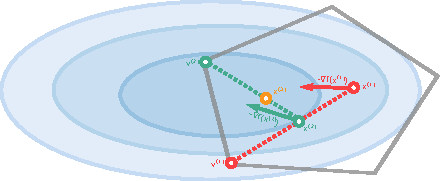
\includegraphics[scale=1.5]{figures/frank_wolfe_cropped.pdf}
    \centering
    \caption{Visual representation of two iterations of Frank-Wolfe. Here the ovals represent the gradient and the pentagon the convex bounds of the problem.}
\end{figure}

\subsection{The \textsc{Fugal} algorithm}
\textsc{Fugal} approximates an optimal alignment of graphs $G_1$ and $G_2$, by constructing an optimisation problem based on \textit{unmediated} representations of the graphs. Based upon the theoretical background described above, we now derive the \textsc{Fugal} algorithm.\\

\noindent
\textbf{QAP Term:} We start with the quadratic assignment problem from Equation \ref{original_qap}:
\begin{equation}
    \min_{P \in \mathds{P}^n} \lVert AP-PB \rVert^2_F
\end{equation} 
where $A$ and $B$ are the adjacency matrices of $G_1$ and $G_2$ respectively. Solving for $P \in \mathds{P}^n$ is NP-hard, as $\mathds{P}^n$ is non-convex \citep{koopmans1957assignment}. By expanding from $P \in \mathds{P}^n$ to the superset $P \in \mathds{W}^n$, where $\mathds{W}^n$ is the set of \textit{doubly stochastic} matrices, a solution can be found using the Frank-Wolfe algorithm \citep{frank1956algorithm}.\\

\noindent
\textbf{LAP Auxiliary Term:} To guide the optimisation, an auxiliary term is derived from NetSimilie \citep{berlingerio2013network} features of the graph nodes. \textsc{Fugal} specifically uses:
\begin{enumerate}
    \item $f_1$: The degree of node $i$.
    \item $f_2$: The clustering coefficient of node $i$.
    \item $f_3$: The average degree of the neighbours of node $i$
    \item $f_4$: The average clustering coefficient of the neighbours of node $i$.
\end{enumerate}

A feature vector $(f_1, f_2, f_3, f_4)$ is constructed for each node. We expect that matching nodes will have similar feature vectors, which is formulated as a LAP:
\begin{equation}
    \lVert F_1 - P F_2 \rVert^2_F 
\end{equation}
where $F_1, F_2 \in \mathds{R}^{n \times 4}$ are the node feature vectors of graph $G_1$ and $G_2$ respectively.\\

\noindent
\textbf{Regularization Term:} To guide the solution towards a permutation matrix, a regularisation term is included:
\begin{equation}
   \text{trace}(P^T(1^{n \times n}-P))  
\end{equation}
which approaches 0 when $P$ approaches the form of a permutation matrix.\\

\noindent
We construct the full optimisation problem:
\begin{equation}\label{full_optimization_problem}
     \min_{P \in \mathds{P}^n} \lVert AP-PB \rVert^2_F + \mu \lVert F_1 - P F_2 \rVert^2_F + \lambda \text{trace}(P^T(1^{n \times n}-P))
\end{equation} 
where $\lambda$ and $\mu$ control the significance of the regularisation and auxiliary term respectively. The regularisation term is non-convex, which makes the problem convex only when $\lambda = 0$.\\

\noindent
\cite{fugal2024} expresses the problem as:
\begin{equation}\label{final_problem}
    \min_{P \in \mathds{W}^n} f(P) + \lambda g(P)
\end{equation}

\noindent
where $f(P) = -\text{trace}(APB^TP^T) + \mu \cdot \text{trace}(P^TD)$ and $g(P) = \text{trace}(P^T(1^{n \times n} - P))$, and $D$ is the Euclidean distance between $F_1$ and $F_2$ as in Equation \ref{euclidean_distance_matrix}. The derivatives are given by:
\begin{equation}\label{sinkhorn-gradient}
    \begin{split}
        \nabla f(P) &= -APB^T - A^TPB + \mu \cdot D\\
        \nabla g(P) &= 1^{n \times n} - 2P
    \end{split}
\end{equation}

\noindent
\textsc{Fugal} optimises Equation \ref{final_problem} repeatedly using the Frank-Wolfe algorithm while increasing $\lambda$. This makes it converge towards a \textit{quasi-permutation} matrix. The linear sub-problem of Frank-Wolfe becomes:
\begin{equation}
     \min_{q\in \mathds{W^n}} \langle \nabla f(P) + \lambda \nabla g(P), q \rangle 
\end{equation}
This is an instance of the optimal transport problem where $r = c = \boldsymbol{1}$, which \textsc{Fugal} efficiently solves using Sinkhorn-Knopp. Lastly, to round to a permutation matrix, \textsc{Fugal} uses the Hungarian algorithm, as this is an instance of LAP.

\begin{algorithm}[H]
\caption{calculate-gradient}\label{alg:calculate-gradient}
\textbf{Input:} $Q \in \mathds{R}^{n \times n}$\\
\textbf{Input:} $\lambda \in \mathds{R}$
\begin{algorithmic}[1]
\State \Return $\nabla f(Q) + \lambda \nabla g(Q)$
\end{algorithmic}
\end{algorithm}

\begin{algorithm}[H]
\caption{find-quasi-permutation}\label{alg:find-quasi-permutation}
\textbf{Input:} $A, B \in \{ 0, 1 \}^{n \times n}$ \Comment{Adjacency matrices of $G_1, G_2$}\\
\textbf{Input:} $D \in \mathds{R}^{n \times n}$ \Comment{Euclidian dist. between $F_1$ and $F_2$}\\
\textbf{Input:} $\mu \in \mathds{R}, T \in \mathds{Z}$
\begin{algorithmic}[1]
\State $Q \gets \boldsymbol{1} \cdot \boldsymbol{1}^T / n$
\For{$\lambda = 0$ \textbf{to} $T - 1$}
    \For{$it$ \textbf{to} $10$} \Comment{Do 10 Frank-Wolfe iterations}
        \State $grad \gets \text{calculate-gradient}(Q, \lambda)$
        \State $q_{it} \gets \text{Sinkhorn-Knopp}(\boldsymbol{1}, \boldsymbol{1}, grad)$
        \State $\alpha \gets \frac{2}{2 + it}$
        \State $Q \gets Q + \alpha(q_{it} - Q)$
    \EndFor
\EndFor
\State \Return $Q$
\end{algorithmic}
\end{algorithm}

\begin{algorithm}[H]
\caption{\textsc{Fugal}}\label{alg:fugal}
\textbf{Input:} Graphs $G_1, G_2$\\
\textbf{Input:} $\mu \in \mathds{R}, T \in \mathds{Z}$
\begin{algorithmic}[1]
\State $F_1, F_2 \gets \text{extract-features}(G_1), \text{extract-features}(G_2)$
\State $D \gets \text{Euclidian-distance}(F_1, F_2)$
\State $Q \gets \text{find-quasi-permutation}(A, B, D, \mu, T)$
\State \Return $\text{Hungarian}(Q)$
\end{algorithmic}
\end{algorithm}

Algorithm \ref{alg:fugal} demonstrates the full \textsc{Fugal} algorithm. First, the two feature matrices $F_1, F_2$ are generated and the Euclidian distance between them is calculated. The \textit{quasi-permutation} matrix is found in Algorithm \ref{alg:find-quasi-permutation}. An initial doubly stochastic matrix $Q$ is defined, where all entries are set to $\frac{1}{n}$. Frank-Wolfe is performed $T$ times, where $\lambda$ is increased for each iteration, increasing the significance of the regularisation term in Algorithm \ref{alg:calculate-gradient}. A fixed number of Frank-Wolfe iterations is run for each $\lambda$. In each iteration, the gradient is calculated, which is then given as input to the Sinkhorn-Knopp algorithm and used to update $Q$. Note that \cite{fugal2024} does not specify the regularisation parameter $\epsilon$ to be used with Sinkhorn-Knopp. Lastly, $Q$ is rounded to a permutation matrix using the Hungarian algorithm to find a maximum assignment with $Q$ as the cost matrix.

\subsection{Runtime analysis of \textsc{Fugal}}
%\cite{fugal2024} proves that 
\textsc{Fugal} runs in $O(n^3)$ for graphs of $n$ nodes. Empirically, we find that the vast majority of the run-time is spent calculating the gradient (Algorithm \ref{alg:calculate-gradient}) and performing Sinkhorn-Knopp iterations (Algorithm \ref{alg:Sinkhorn-Knopp}) (Figure \ref{fig:fugal-scaling}). Unsurprisingly, the execution time of \textsc{Fugal} heavily depends on the amount of Sinkhorn-Knopp iterations required to converge to a doubly stochastic matrix. Here, we also note that the Hungarian algorithm spends more time finding an optimal solution when noise is introduced in the target graph\\

\pgfplotstableread[col sep=comma]{data/fugal_scaling_NSWk10p05.csv}\fsNSW

\begin{figure}
    \centering
\begin{tikzpicture}
\begin{axis}[
    ybar stacked,
    ymin=0,
    xtick=data,
    xticklabels={$2^7$, $2^8$, $2^9$, $2^{10}$, $2^{11}$, $2^{12}$, $2^7$, $2^8$, $2^9$, $2^{10}$, $2^{11}$, $2^{12}$},
    x tick label style={rotate=45},
    legend style={at={(0.5, -0.2)}, anchor=north, legend columns=-1},
    bar width=12pt,
    width=\textwidth*0.66,
    height=\textwidth*0.8,
    xlabel={Number of nodes},
    ylabel={Time (s)},
    ymajorgrids=true,
    xmajorgrids=true,
]
\addplot table[x expr=\coordindex, y index=0] {\fsNSW};
\addplot table[x expr=\coordindex, y index=1] {\fsNSW};
\addplot table[x expr=\coordindex, y index=2] {\fsNSW};
\addplot table[x expr=\coordindex, y index=3] {\fsNSW};
\legend{Sinkhorn-Knopp \ref{alg:Sinkhorn-Knopp}, Feature Extraction, Calculate Gradient \ref{alg:calculate-gradient}, Hungarian}
\end{axis}
\end{tikzpicture}
    \caption{Scaling of \textsc{Fugal} on NW graphs $(k = 8, p = 0.1)$, with no noise and 20\% noise. Time is measured in accumulated wall time for each section. Note that negligible amounts of time is spent outside the measured regions.}
    \label{fig:fugal-scaling}
\end{figure}
